\appendix

% \chapter{Resultados de farmacovigilancia pasiva en Cuba y las Américas}

% \section{Reporte de RAM notificadas por farmacovigilancia pasiva en Cuba}
% \label{app:reportes_cuba_2020}

% En el Anexo~\ref{app:reportes_cuba_2020} se presenta una figura con la evolución de las notificaciones de reacciones adversas a medicamentos (RAM) en Cuba entre 2014 y 2020. Estos datos corresponden al sistema de \textbf{farmacovigilancia pasiva}, basado en la notificación espontánea de sospechas de RAM por parte del personal sanitario.

% \begin{figure}[H]
%     \centering
%     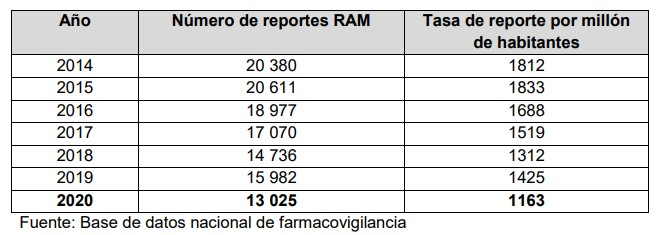
\includegraphics[scale=1.2]{Graphics/Cap1/ram_en_cuba_2020.jpg}
%     \caption{Notificaciones de \gls{reacción adversa a medicamentos (RAM)} declaradas mediante farmacovigilancia pasiva en Cuba (2014-2020). Fuente: \gls{cecmed}, Informe Anual 2020 \cite{cecmed_farmacovigilancia_cuba_2020}.}
%     \label{fig:reporte_ram_cuba_2020}
% \end{figure}

% \section{Reporte según grupo farmacológico}
% \label{app:grupo_farmacologico}

% En el Anexo~\ref{app:grupo_farmacologico} se incluye una figura que muestra los reportes de \gls{reacción adversa a medicamentos (RAM)} según el grupo farmacológico, a partir de la farmacovigilancia pasiva del año 2020.

% \begin{figure}[H]
%     \centering
%     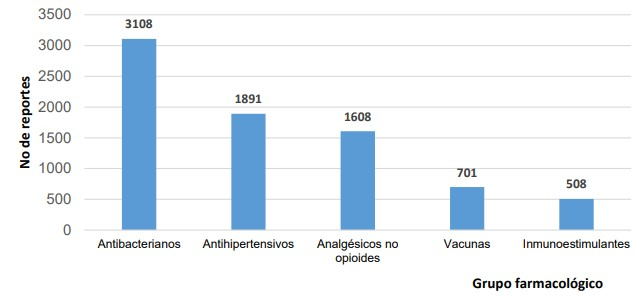
\includegraphics[scale=1.5]{Graphics/Cap1/grupo_farmacologico.jpg}
%     \caption{Reporte de \gls{reacción adversa a medicamentos (RAM)} según grupo farmacológico. Farmacovigilancia pasiva, 2020. Adaptado de \cite{cecmed_farmacovigilancia_cuba_2020}}
%     \label{fig:grupo_farmacologico_ram}
% \end{figure}



% \section{Notificaciones de ESAVI por países de la región de las Américas}
% \label{app:esavi_por_paises}

% En el Anexo~\ref{app:esavi_por_paises} se incluye una figura que presenta el número de \gls{esavi} notificados por los países de la región de las Américas.

% \begin{figure}[H]
%     \centering
%     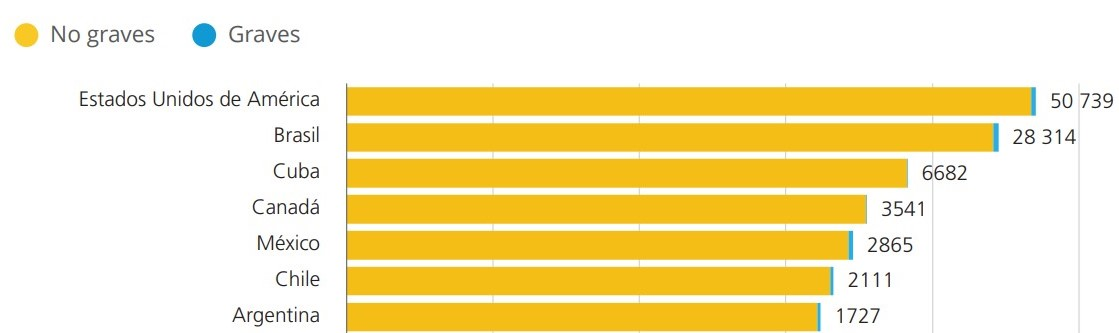
\includegraphics[scale=0.8]{Graphics/Cap1/copia_paises_ram.jpg}
%     \caption{Número de \gls{esavi} notificados por los países de la región de las Américas. Adaptado de \cite{ops_manual_esavi_2021}}
%     \label{fig:esavi_paises_americas}
% \end{figure}

% \section{Estructura del Sistema de Vigilancia de Medicamentos en Cuba}
% \label{app:estructura_vigilancia}

% En el Anexo~\ref{app:estructura_vigilancia} se incluye una figura que presenta la organización del sistema cubano de vigilancia de medicamentos.

% \begin{figure}[htbp]
%     \centering
%     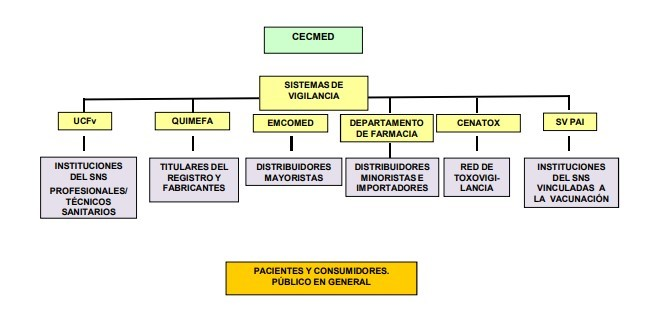
\includegraphics[scale=1.2]{Graphics/Cap1/estructura_vigilancia_medicamentos_cuba2.jpg}
%     \caption{Estructura del Sistema de Vigilancia de Medicamentos en Cuba. Adaptado de: \cite{paho_vigilancia_medicamentos_cuba}}
%     \label{fig:estructura_vigilancia_medicamentos_cuba}
% \end{figure}


% El sistema de vigilancia de medicamentos en Cuba se estructura bajo la rectoría del \gls{cecmed}, autoridad reguladora nacional encargada de la evaluación, control y toma de decisiones sobre la seguridad de los medicamentos a partir de la información generada en el sistema.

% Para el cumplimiento de estas funciones, se articula una red de vigilancia integrada por diversos componentes que interactúan de manera coordinada (ver Figura \ref{fig:estructura_vigilancia_medicamentos_cuba}) \cite{paho_vigilancia_medicamentos_cuba}:

% \begin{itemize} 
%     \item \textbf{\gls{ucnfv} (\gls{minsap}):} Cohesiona la Red de Farmacoepidemiología en los 169 municipios del país y actúa como el canal central para la \gls{notificación espontánea} de profesionales y pacientes, siendo las vacunas la excepción gestionada de forma especializada por el \gls{pai} \cite{paho_vigilancia_medicamentos_cuba,normas_farmacovigilancia_cuba_2012}. 
%     \item \textbf{Fabricantes y Titulares de Registro (QUIMEFA):} Involucra a las 24 empresas farmacéuticas nacionales, donde cada una cuenta con personal designado para la vigilancia y reporta directamente sobre la seguridad y calidad de sus productos \cite{paho_vigilancia_medicamentos_cuba}. 
%     \item \textbf{Distribución Mayorista (EMCOMED):} Coordina la vigilancia en las 24 droguerías del país, detectando problemas de calidad durante el almacenamiento y transportación \cite{paho_vigilancia_medicamentos_cuba}. 
%     \item \textbf{Distribución Minorista (Departamento de Farmacia):} Supervisa la vigilancia en las más de 2,000 farmacias comunitarias y hospitalarias del Sistema Nacional de Salud \cite{paho_vigilancia_medicamentos_cuba}.  
%     \item \textbf{\gls{cenatox}:} Lidera la red de toxicovigilancia, supervisando las intoxicaciones y reacciones adversas de naturaleza \gls{toxica} \cite{paho_vigilancia_medicamentos_cuba}. 
%     \item \textbf{SV \gls{pai}:} Realiza la vigilancia especializada de vacunas mediante el monitoreo de los \gls{esavi}, bajo la supervisión del Viceministerio de Higiene y Epidemiología \cite{paho_vigilancia_medicamentos_cuba}. 
% \end{itemize}

% Toda la información captada por estos efectores fluye hacia el Observatorio de Vigilancia Postcomercialización del \gls{cecmed}, donde se evalúa la relación beneficio-riesgo para emitir alertas farmacológicas, retirar lotes o modificar registros sanitarios en tiempo real \cite{paho_vigilancia_medicamentos_cuba}. 



























% \chapter{Modelos oficiales de notificación en Cuba}
% \label{app:modelos_formularios}

% \section{Modelo 33-36-02}
% \label{app:modelo_33-36-02}

% En el Anexo \ref{app:modelo_33-36-02} se incluye el \textbf{Modelo 33-36-02}, el formulario oficial utilizado por los profesionales de la salud en Cuba para la notificación de sospechas de reacciones adversas a medicamentos dentro del sistema nacional de farmacovigilancia.

% \begin{figure}[H]
%     \centering
%     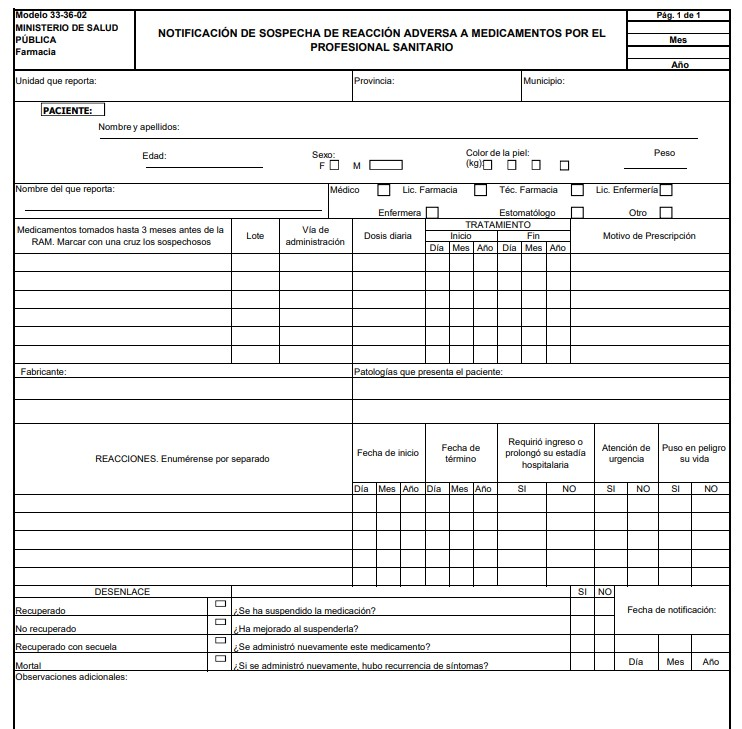
\includegraphics[width=\textwidth]{Graphics/Cap1/modelo_cubano_33_36_02.jpg}
%     \caption{Modelo 33-36-02: Notificación de sospechas de Reacciones Adversas a Medicamentos por el Profesional Sanitario. Adaptado de \cite{normas_farmacovigilancia_cuba_2012}}
% \end{figure}

% % El formulario incluye instrucciones detalladas para la notificación de reacciones adversas, abarcando desde la identificación del medicamento sospechoso hasta la descripción clínica del evento, con el objetivo de garantizar la completitud y calidad de los reportes dentro del sistema de farmacovigilancia.
% \newpage

% \begin{figure}[H]
%     \centering
%     
\includegraphics[width=\textwidth]{Graphics/Cap1/dorso_modelo_33_36_02.jpg}
%     \caption{Instructivo en el dorso del modelo 33-36-02: Notificación de sospechas de Reacciones Adversas a Medicamentos por el Profesional Sanitario, Adaptado de \cite{normas_farmacovigilancia_cuba_2012}}
% \end{figure}

% \newpage

% \section{Modelo 33-36-03}
% \label{app:modelo_33-36-03}

% En el Anexo \ref{app:modelo_33-36-03} se incluye el \textbf{Modelo 33-36-03}, el formulario oficial utilizado por los pacientes en Cuba para la notificación de sospechas de reacciones adversas a medicamentos dentro del sistema nacional de farmacovigilancia.

% \begin{figure}[H]
%     \centering
%     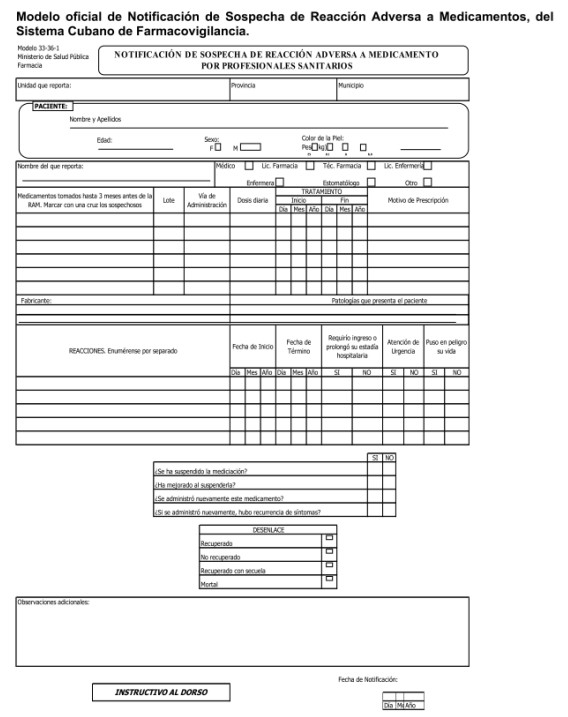
\includegraphics[width=\textwidth]{Graphics/Cap1/modelo_33_36_03.jpg}
%     \caption{Modelo 33-36-03: Notificación de sospechas de Reacciones Adversas a Medicamentos por el Paciente. Adaptado de \cite{normas_farmacovigilancia_cuba_2012}}
% \end{figure}


% \begin{figure}[H]
%     \centering
%     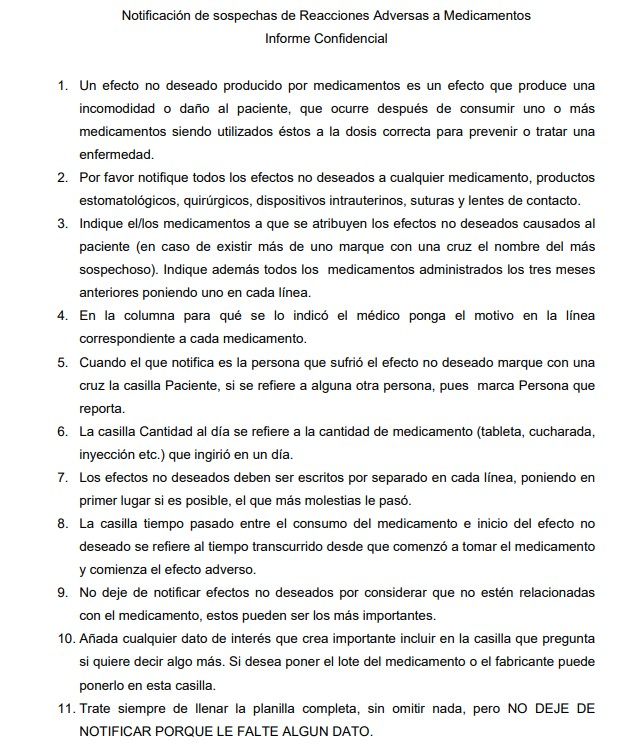
\includegraphics[width=\textwidth]{Graphics/Cap1/dorso_modelo_33_36_03.jpg}
%     \caption{Instructivo en el dorso del modelo 33-36-03: Notificación de sospechas de Reacciones Adversas a Medicamentos por el Paciente. Adaptado de \cite{normas_farmacovigilancia_cuba_2012}}
% \end{figure}


% \newpage

% \section{Modelo 84-30-2}
% \label{app:modelo_84-30-2}
% En el Anexo \ref{app:modelo_84-30-2} se incluye el \textbf{Modelo 84-30-2}, el formulario oficial utilizado por los profesionales de la salud en Cuba para la notificación de sospechas de eventos supuestamente atribuibles a la vacunación o inmunización (ESAVI) dentro del sistema nacional de farmacovigilancia.

% \begin{figure}[H]
%     \centering
%     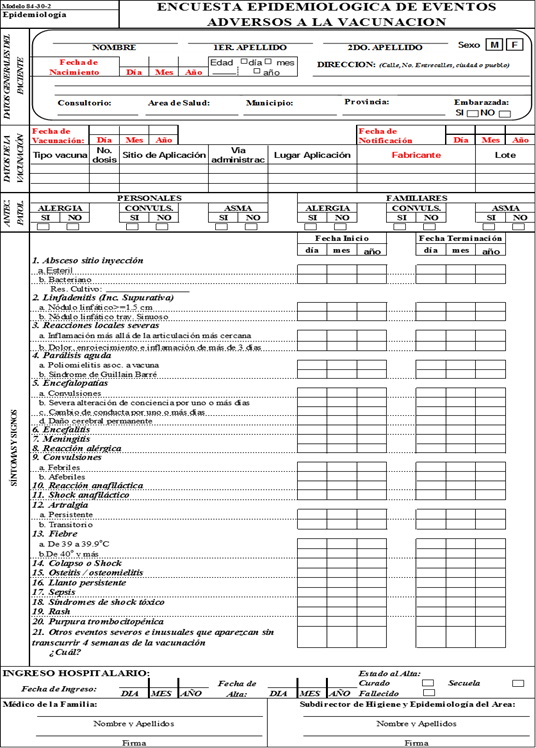
\includegraphics[width=\textwidth]{Graphics/Cap1/modelo_84_30_2.png}
%     \caption{Modelo 84-30-2: Notificación de sospechas de Eventos Supuestamente Atribuibles a la Vacunación o Inmunización (ESAVI). Adaptado de \cite{cecmed_ar_00_515}}
% \end{figure}




% \newpage
% \chapter{Base de Datos Central de Farmacovigilancia (FarmaVigiC)}

% \section{Campos de la base de datos central de farmacovigilancia (FarmaVigiC)}
% \label{app:base_datos_farmavigic}

% En el Anexo \ref{app:base_datos_farmavigic} se describen los campos de la base de datos central de farmacovigilancia (FarmaVigiC) utilizada en Cuba.

% \renewcommand{\arraystretch}{1.3}

% \begin{longtable}{|p{3.2cm}|p{9.3cm}|}
% \caption{Campos de la base de datos central de farmacovigilancia (FarmaVigiC). Elaboración propia a partir de \cite{normas_farmacovigilancia_cuba_2012} (p. 42).}
% \label{tab:base_datos_farmavigic}\\

% \hline
% \textbf{Grupos de campos} & \textbf{Variables o campos} \\
% \hline
% \endfirsthead

% \hline
% \textbf{Grupos de campos} & \textbf{Variables o campos} \\
% \hline
% \endhead
		

% \hline
% \endfoot

		
% 		Paciente & \makecell[l]{Nombre y apellidos\\Edad\\Sexo \\ Raza \\ Antecedentes patológicos personales \\ Requirió ingreso \\ Requirió atención de urgencia \\ Requirió reposo \\ Fue baja laboral o escolar \\ Peligró su vida} \\
%         \hline

%         Notificador & \makecell[l]{Unidad que reporta\\Provincia\\Municipio\\Nombre y apellidos \\ Especialidad} \\
%         \hline

%         Medicamentos & \makecell[l]{Medicamento sospechoso\\Presentación cantidad\\Presentación unidad\\Forma farmacéutica\\Fabricante\\Diluyente\\Lote\\ Vía de administración \\ Dosis cantidad \\ Dosis unidad \\ Dosis frecuencia \\ Fecha de inicio del tratamiento \\ Fecha fin del tratamiento \\ Continuación \\ Motivo de prescripción \\ Otro fármaco 1 \\ Otro fármaco 2 \\ Otro fármaco 3 \\ Otro fármaco 4 \\ Otro fármaco 5 \\ Otro fármaco 6 \\ Vía, dosis, lote de otros fármacos \\ Fecha de administración de otros fármacos} \\
%         \hline

%         Reacciones adversas & \makecell[l]{Reacción principal\\Otra RAM 1\\Otra RAM 2\\Otra RAM 3\\Otra RAM 4\\Otra RAM 5\\Otra RAM 6 \\ Fecha de inicio RAM \\ Fecha fin de RAM \\ Continuación} \\[6pt]
% 		\hline
		
% 		Clasificación & \makecell[l]{Grupo de edades\\Sexo\\Nivel de atención\\Especialidad\\Grupo farmacológico\\Sistema de órgano afectado\\Severidad\\Causalidad\\Importancia\\Frecuencia} \\[6pt]
% 		\hline
		
% 		Desenlace & \makecell[l]{Suspendió la medicación\\Supresión positiva\\Re exposición\\Recurrencia de síntomas\\Desenlace\\Recuperado\\No recuperado \\ Recuperado con secuela} \\[6pt]
% 		\hline

%         Organización e información adicional & \makecell[l]{Mes de entrada a la base\\Secuencia temporal\\Observaciones\\Comentarios\\Resultados de necropsia\\Fecha de notificación} \\[6pt]
% 		\hline

%         Evaluación de la calidad & \makecell[l]{E1 (evalúa al notificador)\\E2 (evalúa al revisor) \\ E3 (evalúa calidad del llenado de la base)} \\[6pt]
% 		\hline
	
% \end{longtable}

% \begin{itemize}
%     \item A nivel municipal se trabajan 71 campos
%     \item A nivel provincial se trabajan 72 campos
%     \item A nivel nacional se trabajan 75 campos
% \end{itemize}

% \newpage

% \chapter{Formularios de referencia}

% \section{Formulario VAERS - Octubre 2025}
% \label{app:vaers-form-oct2025}

% En el Anexo \ref{app:vaers-form-oct2025} se incluye el formulario oficial del Vaccine Adverse Event Reporting System (VAERS) correspondiente a octubre de 2025. Este formulario constituye el instrumento estándar utilizado para la notificación de eventos adversos posteriores a la vacunación en los Estados Unidos.

% \begin{figure}[H]
%     \centering
%     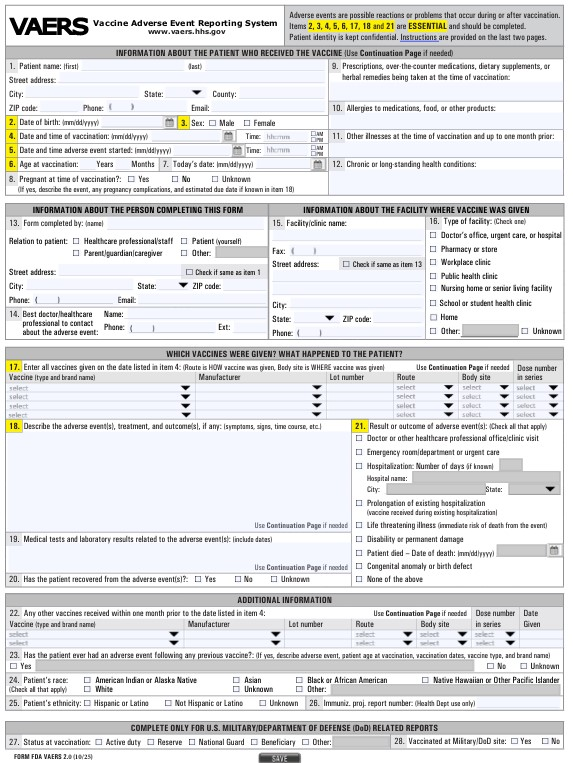
\includegraphics[width=\textwidth]{Graphics/Cap2/vaers-formulario.jpg}
%     \caption{Formulario VAERS - Octubre 2025}
% \end{figure}


% \newpage



% \section{Formulario v-safe - Enero 2021}
% \label{app:vsafe-form-ene2021}

% En el Anexo \ref{app:vsafe-form-ene2021} se incluyen capturas del sistema v-safe del CDC correspondientes a enero de 2021. 
% Este sistema constituye una herramienta de seguimiento activo utilizada para monitorizar síntomas y eventos adversos posteriores a la vacunación.

% \begin{figure}[htpb]
%     \centering
    
%     % Fila 1
%     \begin{minipage}[t]{0.45\textwidth}
%         \centering
%         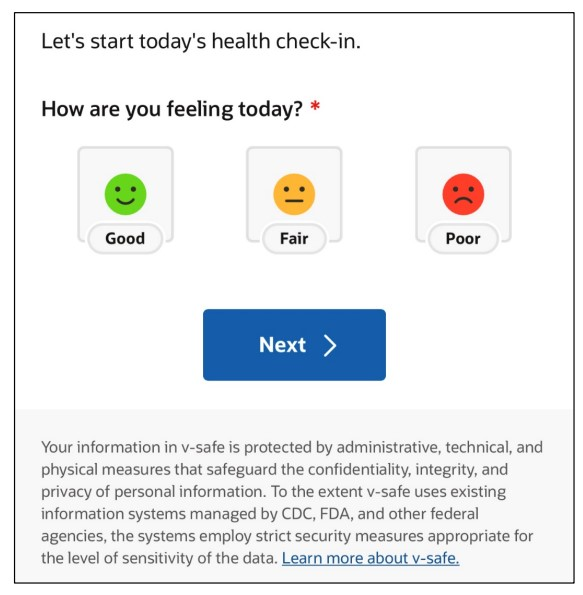
\includegraphics[width=\linewidth]{Graphics/Cap2/feeling.jpg}
%         \caption{Estado general}
%     \end{minipage}
%     \hfill
%     \begin{minipage}[t]{0.45\textwidth}
%         \centering
%         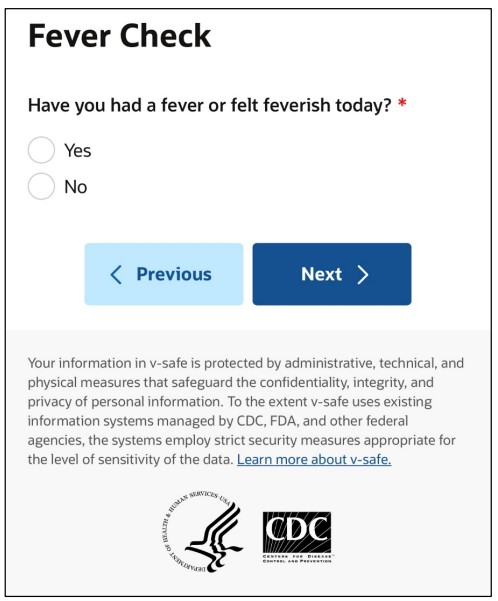
\includegraphics[width=\linewidth]{Graphics/Cap2/fever.jpg}
%         \caption{Verificación de fiebre}
%     \end{minipage}

%     \vspace{0.5cm}
    
%     % Fila 2
%     \begin{minipage}[t]{0.45\textwidth}
%         \centering
%         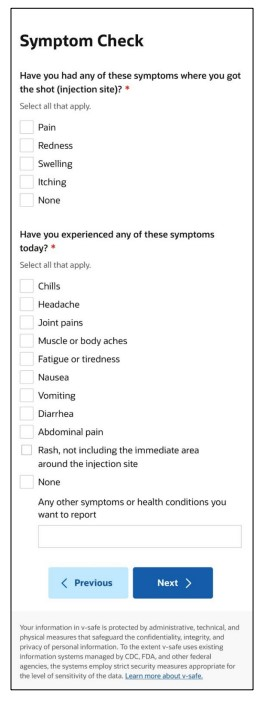
\includegraphics[width=0.5\linewidth]{Graphics/Cap2/symptom.jpg}
%         \caption{Verificación de síntomas}
%     \end{minipage}
%     \hfill
%     \begin{minipage}[t]{0.45\textwidth}
%         \centering
%         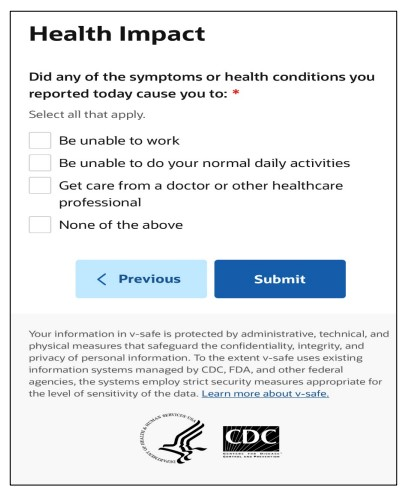
\includegraphics[width=\linewidth]{Graphics/Cap2/health.jpg}
%         \caption{Impacto en la salud}
%     \end{minipage}

%     \caption{Capturas del sistema v-safe para el seguimiento de síntomas posteriores a la vacunación}
%     \label{fig:vsafe-form}
% \end{figure}












% \chapter{Entidades de infraestructura}
% \label{anexo:entidades_infraestructura}

% \section{RefreshToken}

% La entidad \texttt{RefreshToken} permite la renovación de sesiones sin que el usuario deba iniciar sesión nuevamente. Cuando un usuario se autentica, el sistema genera un token de acceso JWT de corta duración y un token de actualización que persiste en esta tabla. Al expirar el token de acceso, el cliente presenta el token de actualización y obtiene uno nuevo.

% \begin{lstlisting}[language={[Sharp]C}, caption={Entidad RefreshToken}, label={lst:refreshtoken}]
% public class RefreshToken : GuidEntity
% {
%     public string Token { get; set; } = null!;
%     public DateTime ExpiresAt { get; set; }
%     public bool Revoked { get; set; }
%     public Guid UserId { get; set; }
%     public User User { get; set; } = null!;
% }
% \end{lstlisting}

% \texttt{Token} almacena el valor del token de actualización. \texttt{ExpiresAt} define su vencimiento. \texttt{Revoked} permite invalidarlo antes de esa fecha. \texttt{UserId} y \texttt{User} asocian cada token con su usuario.


% \section{AuditLog}

% La entidad \texttt{AuditLog} registra las operaciones realizadas sobre el sistema y constituye la base para las funcionalidades de auditoría y trazabilidad descritas en la sección \ref{section:backend} del Capítulo 4. Contempla tanto usuarios autenticados como reporteros anónimos.

% \begin{table}[H]
% \centering
% \caption{Campos de la entidad \texttt{AuditLog}}
% \label{tab:auditlog}
% \begin{tabular}{|l|l|p{6cm}|}
% \hline
% \textbf{Campo} & \textbf{Tipo} & \textbf{Descripción} \\
% \hline
% \texttt{UserId} & \texttt{Guid?} & Usuario autenticado (nulo si es anónimo) \\
% \texttt{UserEmail} & \texttt{string?} & Correo del usuario autenticado \\
% \texttt{ReporterName} & \texttt{string?} & Nombre del reportero anónimo \\
% \texttt{ReporterEmail} & \texttt{string?} & Correo del reportero anónimo \\
% \texttt{Action} & \texttt{string} & Operación: Create, Update, Delete, View \\
% \texttt{EntityName} & \texttt{string} & Entidad afectada (ej. AefiReport) \\
% \texttt{EntityId} & \texttt{Guid?} & Identificador del registro afectado \\
% \texttt{Details} & \texttt{string?} & Descripción legible de la acción \\
% \texttt{OldValues} & \texttt{string?} & Datos antes del cambio (JSON) \\
% \texttt{NewValues} & \texttt{string?} & Datos después del cambio (JSON) \\
% \texttt{IpAddress} & \texttt{string?} & Dirección IP de origen \\
% \texttt{CreatedAt} & \texttt{DateTime} & Fecha y hora de la operación \\
% \hline
% \end{tabular}
% \end{table}




\chapter{Código de las pruebas de rendimiento}
\label{anexo:k6}

A continuación se presentan los scripts de k6 utilizados en las pruebas de rendimiento del Capítulo 5, así como la configuración del entorno de pruebas.

\section{Prueba de carga: creación de reporte ESAVI}
\label{anexo:k6-creacion}

\subsection{Configuración del entorno de prueba}

Cada solicitud de creación incluye: 13 vacunas del Instituto Finlay, 10 lotes por cada vacuna con número de lote, dosis, sitio de administración y fecha; datos del reportante y del paciente generados dinámicamente; y fechas de administración, inicio y fin del evento adverso predefinidas. Para evitar una base de datos completamente vacía, cada prueba se ejecutó con 1000 reportes precargados.

Cada prueba se configuró con etapas de rampa, carga estable y enfriamiento: 1 minuto de subida hasta el objetivo de VUs, 3 minutos de carga estable y 1 minuto de bajada a cero. Las pruebas fueron independientes para cada nivel de carga: 5, 10, 30, 50, 70, 80, 100, 150 y 200 VUs.


\subsection{Script principal (load\_test.js)}

\begin{lstlisting}[language=Java]
import http from 'k6/http';
import { check } from 'k6';
import { buildReport } from './payload.js';

const API_BASE = __ENV.API_BASE || 'http://192.168.XXX.XXX:5137/api';
const TARGET = __ENV.TARGET || 100;

export const options = {
    stages: [
        { duration: '1m', target: Number(TARGET) },
        { duration: '3m', target: Number(TARGET) },
        { duration: '1m', target: 0 },
    ],
};

export default function () {
    const payload = buildReport(__VU, __ITER);

    const res = http.post(
        `${API_BASE}/Report/createPublic`,
        JSON.stringify(payload),
        { headers: { 'Content-Type': 'application/json' } }
    );

    check(res, {
        'status 201': (r) => r.status === 201,
        'tiempo < 3000ms': (r) => r.timings.duration < 3000,
    });
}
\end{lstlisting}

\subsection{Tabla de resultados completos}

La Tabla \ref{tab:anexo-creacion} presenta los valores detallados obtenidos en cada nivel de carga.


\begin{table}[H]
\centering
\caption{Resultados completos de la prueba de carga para creación de reportes.}
\label{tab:anexo-creacion}
\footnotesize
\begin{tabular}{lccccc}
\hline
\textbf{VUs} & \textbf{Latencia (ms)} & \textbf{p(95) (ms)} & \textbf{Lat. sin red (ms)} & \textbf{Throug. (r/s)} & \textbf{<3000ms} \\
\hline
5   & 106.6  & 177.4   & [valor] & 23.1 & 100\% \\
10  & 188.6  & 327.7   & [valor] & 26.8 & 100\% \\
30  & 304.1  & 627.9   & [valor] & 24.6 & 100\% \\
50  & 546.2  & 1192.8  & [valor] & 23.0 & 100\% \\
70  & 975.6  & 2214.1  & [valor] & 20.3 & 100\% \\
80  & 1882.1 & 2956.2  & [valor] & 22.2 & 95.8\% \\
100 & 2246.9 & 4056.4  & [valor] & 20.1 & 74.8\% \\
150 & 4721.3 & 6728.2  & [valor] & 21.0 & 19.1\% \\
200 & 5404.2 & 8011.1  & [valor] & 25.0 & 10.7\% \\
\hline
\end{tabular}
\end{table}


\section{Prueba de carga: búsqueda de reporte ESAVI}
\label{anexo:k6-busqueda}

\subsection{Configuración del Entorno para la Búsqueda}

Las solicitudes de búsqueda seleccionan aleatoriamente un número de notificación de un archivo CSV con identificadores reales, generado para cada tamaño de base de datos (1k, 10k, 50k, 100k). Se empleó la misma configuración de etapas que en la prueba de creación. Los mecanismos de CAPTCHA y limitación por IP se desactivaron temporalmente, ya que las pruebas automatizadas no pueden resolverlos, lo que confirma que estas políticas de seguridad cumplen su función de frenar bots.

\subsection{Script principal (search\_test.js)}

\begin{lstlisting}[language=Java]
import http from 'k6/http';
import { check } from 'k6';
import papaparse from 'https://jslib.k6.io/papaparse/5.1.1/index.js';

const CSV_FILE = __ENV.CSV_FILE || 'reports_1k.csv';
const csvData = papaparse.parse(open(`./${CSV_FILE}`), { header: true }).data;
const BASE_URL = __ENV.API_BASE || 'http://192.168.XXX.XXX:5137/api';
const TARGET = __ENV.TARGET || 10;

export const options = {
    stages: [
        { duration: '1m', target: Number(TARGET) },
        { duration: '3m', target: Number(TARGET) },
        { duration: '1m', target: 0 },
    ],
};

export default function () {
    const registro = csvData[Math.floor(Math.random() * csvData.length)];
    const notificationNumber = registro.notificationNumber;

    const res = http.get(
        `${BASE_URL}/Report/get-report?notificationNumber=${notificationNumber}&token=token-captcha`
    );

    check(res, {
        'status 202': (r) => r.status === 202,
        'tiempo < 3000ms': (r) => r.timings.duration < 3000,
    });
}
\end{lstlisting}

\subsection{Tabla de resultados completos}

La Tabla \ref{tab:anexo-busqueda} presenta los valores detallados obtenidos en cada combinación de tamaño de base de datos y usuarios concurrentes.

\begin{table}[H]
\centering
\caption{Resultados completos de la prueba de carga para búsqueda de reportes.}
\label{tab:anexo-busqueda}
\footnotesize
\begin{tabular}{lccccc}
\hline
\textbf{VUs} & \textbf{BD 1k (ms)} & \textbf{BD 10k (ms)} & \textbf{BD 50k (ms)} & \textbf{BD 100k (ms)} & \textbf{<3000ms} \\
\hline
5   & [valor] & [valor] & [valor] & [valor] & [\%] \\
10  & [valor] & [valor] & [valor] & [valor] & [\%] \\
30  & [valor] & [valor] & [valor] & [valor] & [\%] \\
50  & [valor] & [valor] & [valor] & [valor] & [\%] \\
100 & [valor] & [valor] & [valor] & [valor] & [\%] \\
\hline
\end{tabular}
\end{table}

\section{Prueba de carga: escenario combinado}
\label{anexo:k6-combinado}

\subsection{Configuración del entorno}

El escenario combinado integra los tres perfiles de uso del sistema en una sola prueba: tráfico público (75 VUs, alternando 65\% creación de reportes y 35\% búsqueda por notificación, con pausas de 1 a 3 segundos), tráfico de jefes municipales (10 VUs, consultando el dashboard y asignando reportes a médicos, con pausas de 2 a 6 segundos) y tráfico de médicos (15 VUs, revisando su bandeja de asignaciones y evaluando reportes, con pausas de 1 a 4 segundos). Las pausas simulan el comportamiento humano real y evitan la saturación artificial. Las métricas se aislaron mediante tags para obtener resultados independientes por cada tipo de operación.

Los mecanismos de CAPTCHA y limitación por IP se desactivaron temporalmente por las mismas razones expuestas en la prueba de búsqueda.

\subsection{Ejecución y procesamiento}

La prueba se ejecutó con el siguiente comando, generando dos archivos de salida:

\begin{verbatim}
k6 run --out json=raw.json --summary-export=summary.json mixted2.js
\end{verbatim}

El archivo \texttt{summary.json} contiene las métricas agregadas que el ecosistema de k6 calcula automáticamente: promedio, mediana, p(95), mínimo, máximo y número de solicitudes por cada tag definido. El archivo \texttt{raw.json} registra cada solicitud individual con su latencia y tag asociado. Este archivo crudo se procesó con un script de Python para calcular las métricas adicionales requeridas por los diagramas de caja: cuartiles (Q1, Q3) y valores atípicos (outliers), definidos como aquellas solicitudes cuya latencia supera Q3 + 1.5 $\times$ (Q3 $-$ Q1).

\subsection{Script principal (mixted2.js)}

\begin{lstlisting}[language=Java]
import http from 'k6/http';
import { check, sleep } from 'k6';
import papaparse from './papaparse.js';
import { buildReport } from './create_report/base.js';

const BASE_URL = 'http://192.168.XXX.XXX:5137/api';
const csvData = papaparse.parse(open('./reports_1k.csv'), { header: true }).data;

const DASHBOARD_ENDPOINTS = [
    '/MunicipalDashboard/overview',
    '/MunicipalDashboard/doctors-performance',
    '/MunicipalDashboard/stats_municipal',
];

export const options = {
    scenarios: {
        trafico_publico: {
            executor: 'constant-vus',
            vus: 75,
            duration: '1m',
            exec: 'escenarioPublico',
        },
        trafico_jefes: {
            executor: 'constant-vus',
            vus: 10,
            duration: '1m',
            exec: 'escenarioJefes',
        },
        trafico_medicos: {
            executor: 'constant-vus',
            vus: 15,
            duration: '1m',
            exec: 'escenarioMedicos',
        },
    },
    thresholds: {
        'http_req_duration{name:CrearReporte}': ['p(95)<3000'],
        'http_req_duration{name:BuscarReporte}': ['p(95)<3000'],
        'http_req_duration{name:Dashboard_jefe}': ['p(95)<4000'],
        // resto de thresholds por cada nombre relevante
    },
};

export function escenarioPublico() {
    const rand = Math.random();
    if (rand < 0.65) {
        const createReport = buildReport(__ITER);
    } else {
        const getReport = getReport(_ITER);
    }
    sleep(Math.random() * 2 + 1);
}

export function escenarioJefes() {
    const rand = Math.random();

    if (rand < 0.65) {
        // Obtener reportes pendientes y evaluadores
        const pendingRes = getReportsPendings(__ITER);

        // asignar
        const assignRes = assignReportToDoctor(__ITER);
    } else {
        const resDashboard = getDashboardData(__ITER);
    }
    sleep(Math.random() * 4 + 2);
}

export function escenarioMedicos() {

    // buscar las asignaciones
    const assignments = getMyAssignments(__ITER);

    // evaluar
    const evalRes = evaluateReport(__ITER, assignments);

    sleep(Math.random() * 3 + 1);
}
\end{lstlisting}

\subsection{Tabla de resultados completos}

La Tabla \ref{tab:anexo-combinado} presenta las métricas detalladas obtenidas para cada operación en el escenario combinado.

\begin{table}[H]
\centering
\caption{Resultados completos del escenario combinado con 100 VUs.}
\label{tab:anexo-combinado}
\footnotesize
\begin{tabular}{lcccccccc}
\hline
\textbf{Métrica} & Crear & Buscar & Pendientes & Médicos & Asignar & Asignaciones & Evaluar & Dashboard \\
\hline
Solicitudes & 1078 & 581 & 84 & 84 & 84 & 365 & 68 & 38 \\
Promedio (ms) & 1021.37 & 268.04 & 423.15 & 275.19 & 603.64 & 348.86 & 433.61 & 428.00 \\
Mediana (ms) & 858.28 & 235.99 & 364.01 & 222.53 & 433.23 & 278.22 & 382.17 & 368.06 \\
Q1 (ms) & 616.87 & 157.37 & 223.25 & 153.75 & 291.09 & 180.81 & 276.81 & 208.54 \\
Q3 (ms) & 1170.59 & 324.28 & 484.20 & 358.44 & 626.59 & 427.35 & 515.97 & 480.45 \\
p(95) (ms) & 2468.39 & 551.48 & 1143.59 & 637.15 & 1805.32 & 783.83 & 911.90 & 1209.34 \\
Mínimo (ms) & 151.15 & 24.89 & 68.61 & 54.73 & 101.22 & 46.62 & 81.17 & 60.88 \\
Máximo (ms) & 4389.06 & 1389.79 & 1320.05 & 887.75 & 2571.61 & 1928.12 & 1262.24 & 1255.79 \\
Outliers & 80 & 25 & 8 & 4 & 12 & 18 & 4 & 4 \\
\% éxito & 100\% & 100\% & 100\% & 100\% & 100\% & 100\% & 100\% & 100\% \\
\hline
\end{tabular}
\end{table}

\section{Resultados completos de la auditoría Lighthouse}
\label{anexo:lighthouse}

La Tabla \ref{tab:anexo-categorias} resume los puntajes por categoría para todas las páginas del sistema. En cada celda, el valor superior corresponde al entorno de escritorio y el inferior al móvil.


\begin{table}[H]
\centering
\caption{Puntajes generales de Lighthouse para todas las páginas del sistema.}
\label{tab:anexo-categorias}
\footnotesize
\begin{tabular}{lcccc}
\hline
\textbf{Página} & \textbf{Rendimiento} & \textbf{Accesibilidad} & \textbf{Recomendaciones} & \textbf{SEO} \\
\hline
Página principal (E)   & 100 & 98 & \multirow{2}{*}{96} & \multirow{2}{*}{91} \\
Página principal (M)   & 90  & 93 & & \\ \hline
Registro de ESAVI (E)  & 100 & 89 & \multirow{2}{*}{96} & \multirow{2}{*}{91} \\
Registro de ESAVI (M)  & 96  & 89 & & \\ \hline
Panel informativo (E)  & 100 & 98 & \multirow{2}{*}{96} & \multirow{2}{*}{91} \\
Panel informativo (M)  & 95  & 95 & & \\ \hline
Consulta de reportes (E) & [ ] & [ ] & \multirow{2}{*}{96} & \multirow{2}{*}{91} \\
Consulta de reportes (M) & [ ] & [ ] & & \\ \hline
Gestión de reportes (E)  & [ ] & [ ] & \multirow{2}{*}{96} & \multirow{2}{*}{91} \\
Gestión de reportes (M)  & [ ] & [ ] & & \\ \hline
Gestión de médicos (E)   & [ ] & [ ] & \multirow{2}{*}{96} & \multirow{2}{*}{91} \\
Gestión de médicos (M)   & [ ] & [ ] & & \\ \hline
Gestión de jefes (E)     & [ ] & [ ] & \multirow{2}{*}{96} & \multirow{2}{*}{91} \\
Gestión de jefes (M)     & [ ] & [ ] & & \\ \hline
Gestión de catálogo (E)  & 100 & 94 & \multirow{2}{*}{100} & \multirow{2}{*}{91} \\
Gestión de catálogo (M)  & 95 & 94 & & \\ \hline
Dashboard municipal (E)  & [ ] & [ ] & \multirow{2}{*}{96} & \multirow{2}{*}{91} \\
Dashboard municipal (M)  & [ ] & [ ] & & \\ \hline
Inicio de sesión (E)     & [ ] & [ ] & \multirow{2}{*}{96} & \multirow{2}{*}{91} \\
Inicio de sesión (M)     & [ ] & [ ] & & \\ \hline
\multicolumn{5}{l}{\footnotesize (E) = Escritorio, (M) = Móvil. Mejores Prácticas y SEO son uniformes en todas las páginas.} \\
\end{tabular}
\end{table}

La Tabla \ref{tab:anexo-rendimiento} presenta las métricas de rendimiento detalladas para todas las páginas del sistema.

\begin{table}[H]
\centering
\caption{Métricas de rendimiento para todas las páginas del sistema.}
\label{tab:anexo-rendimiento}
\footnotesize
\begin{tabular}{lcccccccc}
\hline
\textbf{Página} & \textbf{Puntaje} & \textbf{FCP} & \textbf{LCP} & \textbf{TBT} & \textbf{SI} & \textbf{CLS} \\
 & E / M & E / M & E / M & E / M & E / M & E / M \\
\hline
Página principal &
    \makecell{100 \\ 90} &
    \makecell{0.4 s \\ 2.2 s} &
    \makecell{0.6 s \\ 2.9 s} &
    \makecell{0 ms \\ 0 ms} &
    \makecell{0.7 s \\ 4.6 s} &
    \makecell{0.00 \\ 0.00} \\
% \hline
% Registro de ESAVI &
%     \makecell{100 \\ 96} &
%     \makecell{0.4 s \\ 1.7 s} &
%     \makecell{0.6 s \\ 2.7 s} &
%     \makecell{0 ms \\ 0 ms} &
%     \makecell{0.6 s \\ 1.7 s} &
%     \makecell{0.00 \\ 0.00} \\
% \hline
% Panel informativo &
%     \makecell{100 \\ 95} &
%     \makecell{0.4 s \\ 1.7 s} &
%     \makecell{0.6 s \\ 2.4 s} &
%     \makecell{0 ms \\ 0 ms} &
%     \makecell{0.5 s \\ 3.9 s} &
%     \makecell{0.00 \\ 0.00} \\
% \hline
% Consulta de reportes &
%     \makecell{[ ] \\ [ ]} &
%     \makecell{[ ] \\ [ ]} &
%     \makecell{[ ] \\ [ ]} &
%     \makecell{[ ] \\ [ ]} &
%     \makecell{[ ] \\ [ ]} &
%     \makecell{[ ] \\ [ ]} \\
% \hline
% Gestión de reportes &
%     \makecell{[ ] \\ [ ]} &
%     \makecell{[ ] \\ [ ]} &
%     \makecell{[ ] \\ [ ]} &
%     \makecell{[ ] \\ [ ]} &
%     \makecell{[ ] \\ [ ]} &
%     \makecell{[ ] \\ [ ]} \\
% \hline
% Gestión de médicos &
%     \makecell{[ ] \\ [ ]} &
%     \makecell{[ ] \\ [ ]} &
%     \makecell{[ ] \\ [ ]} &
%     \makecell{[ ] \\ [ ]} &
%     \makecell{[ ] \\ [ ]} &
%     \makecell{[ ] \\ [ ]} \\
% \hline
% Gestión de jefes &
%     \makecell{[ ] \\ [ ]} &
%     \makecell{[ ] \\ [ ]} &
%     \makecell{[ ] \\ [ ]} &
%     \makecell{[ ] \\ [ ]} &
%     \makecell{[ ] \\ [ ]} &
%     \makecell{[ ] \\ [ ]} \\
\hline
Gestión de catálogo &
    \makecell{100 \\ 95} &
    \makecell{0.4 s \\ 1.8 s} &
    \makecell{0.4 s \\ 2.6 s} &
    \makecell{0 ms \\ 70 ms} &
    \makecell{0.6 s \\ 2.9 s} &
    \makecell{0.029 \\ 0.00} \\
% \hline
% Dashboard municipal &
%     \makecell{[ ] \\ [ ]} &
%     \makecell{[ ] \\ [ ]} &
%     \makecell{[ ] \\ [ ]} &
%     \makecell{[ ] \\ [ ]} &
%     \makecell{[ ] \\ [ ]} &
%     \makecell{[ ] \\ [ ]} \\
% \hline
% Inicio de sesión &
%     \makecell{[ ] \\ [ ]} &
%     \makecell{[ ] \\ [ ]} &
%     \makecell{[ ] \\ [ ]} &
%     \makecell{[ ] \\ [ ]} &
%     \makecell{[ ] \\ [ ]} &
%     \makecell{[ ] \\ [ ]} \\
\hline
\multicolumn{8}{l}{\footnotesize En cada celda: valor superior = Escritorio (E), valor inferior = Móvil (M).} \\
\end{tabular}
\end{table}